\documentclass[aspectratio=1610]{beamer}
\hypersetup{
    unicode=true,
    linkcolor=blue,
    anchorcolor=blue,
    citecolor=green,
    filecolor=black,
    urlcolor=blue
}

\usepackage{amsmath}
\usepackage{amssymb}
\usepackage{booktabs}
\usepackage{textcomp}
\usepackage{graphicx}
\graphicspath{{figures/}}

\usepackage[style=authoryear,backend=biber]{biblatex}
\addbibresource{references.bib}

%%%%%%%%%%%%%%%%%%%%%%%%%%%%%%%%%%%
%% Minimal clean Beamer style -- no outer theme, single slim footer

\usetheme{default}
\useinnertheme{circles}
\usefonttheme{serif}

%% -- Remove navigation symbols -----------------------------------------------
\setbeamertemplate{navigation symbols}{}

%% -- Frame title with hairline rule ------------------------------------------
\setbeamertemplate{frametitle}{%
  \vskip2pt%
  \usebeamerfont{frametitle}\insertframetitle\strut%
  \vskip-1pt%
  \leaders\vrule width \textwidth\vskip0.4pt%
  \vskip3pt%
  \nointerlineskip
}

%% -- Slim footer: short title (left) + page/total (right) --------------------
\setbeamercolor{footline slim}{fg=gray!70}

\setbeamertemplate{footline}{%
  \leavevmode%
  \hbox{%
    \begin{beamercolorbox}[wd=.70\paperwidth,ht=2ex,dp=1ex,left]{footline slim}%
      \hspace*{2ex}{\tiny\color{gray!70}%
        F.~Guidetti \quad \insertshorttitle}%
    \end{beamercolorbox}%
    \begin{beamercolorbox}[wd=.30\paperwidth,ht=2ex,dp=1ex,right]{footline slim}%
      {\tiny\color{gray!70}\insertframenumber\,/\,\inserttotalframenumber}%
      \hspace*{2ex}%
    \end{beamercolorbox}%
  }%
  \vskip0pt%
}
%%%%%%%%%%%%%%%%%%%%%%%%%%%%%%%%%%%%%%%%%%%%%%%%


\title[Three-Layer Commodity Price Analysis]{A Three-Layer Analysis of Commodity Price Distributions\\Under Geopolitical Stress}
\subtitle{Evidence from Middle East Escalation Scenarios}
\author[F.~Guidetti]{Francesco Guidetti}
\date{April 2026}

\begin{document}

% ── Title ──────────────────────────────────────────────────────────────────────
\begin{frame}[plain]
  \titlepage
\end{frame}

\begin{frame}[shrink=20]{Outline}
  \tableofcontents[hideallsubsections]
\end{frame}

% ══════════════════════════════════════════════════════════════════════════════
\section{Introduction \& Motivation}
% ══════════════════════════════════════════════════════════════════════════════

% ── Slide 1.1 ─────────────────────────────────────────────────────────────────
\subsection{The 2026 Iran War Commodity Shock}

\begin{frame}[shrink=15]{Iran War Shock: Geopolitical Risk and Commodity Prices}

  \small
  The Strait of Hormuz is the world's single most critical commodity choke-point:
  ${\sim}$21\,million\,bbl/day of crude \& products (${\approx}$21\% of global
  supply) plus ${\sim}$10\,bcf/day of LNG (\~20\% of global LNG trade) pass through a 33\,km-wide passage.
  A partial closure in late February~2026 triggered a cascade across four
  sectors: \textbf{energy $\to$ fertilizer $\to$ food}, with metals exposed
  independently via energy-intensive smelting and freight disruption.
  \normalsize

  \medskip
  \begin{center}
  \small
  \textbf{Commodity Prices Surge since Strait of Hormuz Shock}\\[3pt]
  \begin{tabular}{lp{3.8cm}p{4.8cm}}
    \toprule
    \textbf{Sector} & \textbf{March 2026 Change} & \textbf{Threatened Exposure} \\
    \midrule
    Energy       & Crude +41\%, Brent +46\%, TTF +59\%, LNG +31\%& Power generation, transport, petrochemicals \\
    Fertilizers  & DAP +5\%
                 & Global grain production\\
    Agriculture  & Wheat +7\%, Maize +2\%
                 & Food-importing nations; livestock feed chains \\
    Metals       & Aluminium +10\%
                 & Energy-intensive smelting; Hormuz freight routes \\
    \bottomrule
  \end{tabular}
  \end{center}

  \begin{footnotesize}
    \textit{Source:} World Bank Pink Sheet (updated April~2, 2026).
    Monthly average price change February $\to$ March 2026.
  \end{footnotesize}

\end{frame}

% ── Slide 1.2 ─────────────────────────────────────────────────────────────────
\subsection{Analytical Framework}

\begin{frame}[shrink=15]{Analysing the Shock: A Three-Layer Decomposition}

  \medskip
  \textbf{Three separable, estimable layers:}

  \medskip
  \begin{tabular}{llp{4.5cm}}
    \toprule
    Layer & Model & What it adds \\
    \midrule
    Mean $\mu_{i,t}$        & ARX-Koyck + sparse network & GPR-conditional price path; cross-commodity propagation\\
    Variance $\sigma_{i,t}$ & GJR-GARCH  & Asymmetric volatility dynamics\\
    Correlation $\bar{R}$   & DCC-MIDAS  & Shock co-movement\\
    \bottomrule
  \end{tabular}

  \medskip
  \begin{alertblock}{}
    $f(\mathbf{P}_{t+h} \mid \mathrm{GPR}_t)$ decomposes into three estimable
    objects: a conditional mean (ARX-Koyck), a conditional variance
    (GJR-GARCH), and a conditional correlation (DCC-MIDAS). Each layer is
    independently identified and separately interpretable.
  \end{alertblock}

\end{frame}

% ══════════════════════════════════════════════════════════════════════════════
\section{Data}
% ══════════════════════════════════════════════════════════════════════════════

% ── Slide 2.1 ─────────────────────────────────────────────────────────────────
\subsection{Data Sources and Estimation Sample}

\begin{frame}[shrink=20]{Data Sources}

\textbf{Commodity Prices --- World Bank Pink Sheet}\\[4pt]
14 series chosen for direct Strait of Hormuz exposure; monthly nominal USD, 1960--2026.\\[8pt]
\medskip
\begin{tabular}{ll}
    \toprule
    Group        & Series \\
    \midrule
    Energy       & Crude Oil, Brent, NatGas US, NatGas EU, LNG Japan, Coal AU \\
    Fertilizers  & Urea, DAP, TSP, Phosphate Rock \\
    Agriculture  & Wheat, Maize \\
    Metals       & Copper, Aluminum \\
    \bottomrule
  \end{tabular}

  \medskip

  \textbf{GPR Index --- Caldara--Iacoviello \parencite{caldara_measuring_2022}}\\[4pt]
  Monthly, 1985--2026.

  \medskip
  \textbf{Trade Balance --- UN Comtrade}\\[4pt]
  Bilateral flows 2021--2023 (three-year average).

\end{frame}


% ══════════════════════════════════════════════════════════════════════════════
\section{The GPR Index}
% ══════════════════════════════════════════════════════════════════════════════

% ── Slide 2.1 ─────────────────────────────────────────────────────────────────
\subsection{Caldara--Iacoviello Construction: Threats vs Acts}

\begin{frame}[shrink=10]{The GPR Index: Threats vs Acts \parencite{caldara_measuring_2022}}

\begin{itemize}
  \item \textbf{GPR}: share of newspaper articles mentioning geopolitical tension,
          normalized to average 100 over the 1985--2019 period; monthly, 1985--present
\end{itemize}

\smallskip

\begin{columns}[T]
\column{0.48\textwidth}
\textbf{GPRT --- Geopolitical Threats}\\[6pt]
Forward-looking escalation risk: war risk, military mobilization,
nuclear mentions.\\[6pt]
Captures \emph{risk premia} and precautionary demand.

\column{0.48\textwidth}
\textbf{GPRA --- Geopolitical Acts}\\[6pt]
Realized events: military operations, terrorist attacks.\\[6pt]
Captures \emph{demand destruction} and recession fears.
\end{columns}

\medskip

  \begin{center}
  \small
  \textbf{Historical anchors}\\
  \smallskip
  \begin{tabular}{@{}lcc@{}}
    \toprule
    Event                     & GPRT & GPRA \\
    \midrule
    9/11 --- 2001             & $\approx 180$ & $\approx 410$ \\
    Iraq War --- 2003         & $\approx 222$ & $\approx 130$ \\
    Ukraine --- Feb 2022      & $\approx 200$ & $\approx 180$ \\
    \textbf{Iran War Mar 2026}& $\mathbf{293}$ & $\mathbf{404}$ \\
    \bottomrule
  \end{tabular}
  \end{center}
\end{frame}
% ══════════════════════════════════════════════════════════════════════════════
\section{Commodity Price Model (ARX-Koyck)}
% ══════════════════════════════════════════════════════════════════════════════

% ── Slide 4.1 ─────────────────────────────────────────────────────────────────
\subsection{The Koyck ARX Equation}

\begin{frame}[shrink=10]{The ARX-Koyck Model}

  For each commodity $i$, monthly log-returns:

  \begin{align*}
    \Delta \log P_{i,t} &= \alpha_i
      + \phi_i \Delta \log P_{i,t-1}
      + \kappa_i^T \Delta \mathrm{GPRT}_t^*
      + \delta_i^T \mathrm{GPRT}_{t-1}^* \\
    &\phantom{{}={}}
      + \kappa_i^A \Delta \mathrm{GPRA}_t^*
      + \delta_i^A \mathrm{GPRA}_{t-1}^*
      + \sum_j \beta_{ij} \Delta \log P_{j,t-1}
      + \varepsilon_{i,t}
  \end{align*}

  \textbf{Koyck reparameterization --- two distinct GPR effects:}
  \begin{itemize}
    \item $\kappa_i^T$: coefficient on $\Delta\mathrm{GPRT}_t^*$ ---
          immediate price response to a \emph{new} GPR surprise this month
    \item $\delta_i^T$: coefficient on $\mathrm{GPRT}_{t-1}^*$ ---
          effect of the \emph{sustained level} of geopolitical tension
  \end{itemize}

  \textbf{Empirical finding:} $\delta_i \approx 0$ for most commodities ---
  prices respond to GPR \emph{news} ($\Delta$GPRT), not a permanently
  elevated index level. Exception: crude oil and Brent show a small but
  significant negative level effect ($\hat{\delta}^T = -0.025^{***}$),
  consistent with market normalisation under prolonged tension.

  \begin{alertblock}{The $\kappa$ terms are the scenario engine}
    They differentiate De-escalation, Baseline, and Escalation because each
    scenario generates a different GPRT path and therefore a different monthly
    sequence of $\Delta\mathrm{GPRT}$. Without the Koyck impulse, all three
    scenarios produce near-identical mean paths.
  \end{alertblock}

\end{frame}

% ── Slide 4.2 ─────────────────────────────────────────────────────────────────
\subsection{Sparse Network Extension}

\begin{frame}[shrink=10]{Sparse Cross-Commodity Price Network}

  \begin{itemize}
    \item Each commodity may load on lagged returns of other commodities ---
          the cross-beta matrix $\{\beta_{ij}\}$ is selected by BIC stepwise
    \item BIC penalizes additional parameters, retaining only cross-lags with
          genuine predictive content
  \end{itemize}

  \smallskip

  \textbf{Key selected links} (all $p < 0.01$):

  \begin{tabular}{lc}
    \toprule
    Link & $\hat{\beta}_{ij}$ \\
    \midrule
    TSP $\leftarrow$ DAP        & $+0.299$ \\
    DAP $\leftarrow$ TSP        & $+0.262$ \\
    TSP $\leftarrow$ Copper     & $+0.169$ \\
    DAP $\leftarrow$ Aluminum   & $+0.168$ \\
    Phosphate $\leftarrow$ TSP  & $+0.274$ \\
    \bottomrule
  \end{tabular}

  \smallskip

  \begin{alertblock}{Fertilizer indirect channel}
    Fertilizer $\kappa^T$ is not significant --- their GPR sensitivity runs
    entirely through the energy-metals-fertilizer network.
    The DAP--TSP mutual feedback ($\lambda_1 = 0.76$, stable) is the primary
    amplification channel.
  \end{alertblock}

\end{frame}

% ── Slide 4.3 ─────────────────────────────────────────────────────────────────
\subsection{Estimation Results}

\begin{frame}[shrink=10]{Estimation Results: GPR Coefficients}

  \textbf{Energy commodities:}

  \[
    \begin{array}{lcccccc}
      
       & \hat{\phi} & \hat{\kappa}^T & \hat{\delta}^T & \hat{\kappa}^A & \hat{\delta}^A & \hat{\sigma} \\
    \text{CrudeOil} & 0.288^{***} & 0.028^{***} & -0.025^{***} & -0.024^{***} & 0.016^{**}  & 0.087 \\
      \text{Brent}    & 0.253^{***} & 0.028^{***} & -0.025^{***} & -0.024^{***} & 0.015^{**}  & 0.089 \\
      \text{NatGas US}& 0.016       & 0.010       & -0.007       & -0.028^{**}  & 0.024^{**}  & 0.146 \\
      \text{NatGas EU}& 0.271^{***} & 0.011       & -0.008       &  0.002       & -0.007      & 0.092 \\
      \text{LNG Japan}& 0.341^{***} & -0.005      &  0.005       &  0.004       & -0.005      & 0.047 \\
      \text{Coal AU}  & 0.271^{***} &  0.008      & -0.003       & -0.004       & -0.001      & 0.068 \\
    \end{array}
  \]

  \medskip
  
\begin{alertblock}{Buy the rumor, sell the news}
For crude oil and Brent: $\hat{\kappa}^T > 0$ (threats raise prices via
risk premium) and $\hat{\kappa}^A < 0$ (realized acts lower them via demand
destruction). GPRA $= 404$ in March 2026 already signals the ``sell the news''
dynamic: the conflict has materialized, shifting the dominant channel from
risk premium to demand-destruction.
\end{alertblock}
\end{frame}

% ── Slide 4.4b ────────────────────────────────────────────────────────────────
\subsection{GPR Coefficients: Other Commodities}

\begin{frame}[shrink=10]{Estimation Results: GPR Coefficients (Other Commodities)}

  {\small
  \[
    \begin{array}{lcccccc}
       & \hat{\phi} & \hat{\kappa}^T & \hat{\delta}^T & \hat{\kappa}^A & \hat{\delta}^A & R^2 \\
      \text{Urea}      & 0.1466^{***} & -0.0068        &  0.0091        &  0.0072        & -0.0080        & 0.024 \\
      \text{DAP}       & 0.4331^{***} &  0.0046        & -0.0007        &  0.0001        & -0.0010        & 0.192 \\
      \text{TSP}       & 0.5222^{***} &  0.0062        & -0.0015        & -0.0039        &  0.0016        & 0.278 \\
      \text{Phosphate} & 0.2228^{***} & -0.0045        &  0.0064        &  0.0010        & -0.0044        & 0.052 \\
      \text{Wheat}     & 0.2331^{***} &  0.0058        & -0.0044        & -0.0035        &  0.0042        & 0.056 \\
      \text{Maize}     & 0.2722^{***} &  0.0086^{*}    & -0.0067        & -0.0081^{*}    &  0.0062        & 0.080 \\
      \text{Copper}    & 0.3778^{***} &  0.0070        & -0.0062        & -0.0074        &  0.0079^{*}    & 0.149 \\
      \text{Aluminum}  & 0.1872^{***} &  0.0123^{***}  & -0.0076^{*}    & -0.0077^{*}    &  0.0051        & 0.052 \\
    \end{array}
  \]
  }

  \begin{alertblock}{Fertilizers: no direct GPR channel}
    Urea, DAP, TSP show no significant $\hat{\kappa}^T$ or $\hat{\kappa}^A$ ---
    their price channel runs entirely through energy costs via the network, not
    geopolitical news. Aluminum responds strongly to threats ($p = 0.003$).
    Maize shows marginal significance on both GPRT and GPRA.
  \end{alertblock}

\end{frame}

% ── Slide 4.5 ─────────────────────────────────────────────────────────────────
\subsection{BIC Model Comparison}

\begin{frame}[shrink=30]{BIC Model Comparison}

  \medskip

  {\scriptsize
  \begin{tabular}{llrrrrrr}
    \toprule
    Group & Commodity & AR(1) & Koyck-ARX & +Network & $\Delta$BIC & LR $p$ & GPR sig.\\
    \midrule
    Energy & Crude Oil  & $-970.0$ & $-966.0$ & $-968.7$           & $-2.6$           & $0.0002^{***}$ & \checkmark \\
    Energy & Brent      & $-941.3$ & $-933.8$ & $-936.6$           & $-2.9$           & $0.0004^{***}$ & \checkmark \\
    Energy & NatGas US  & $-472.3$ & $-463.6$ & $-473.7$           & $-10.1$          & $0.1921$       & \checkmark \\
    Energy & NatGas EU  & $-929.8$ & $-903.4$ & $\mathbf{-920.1}$  & $\mathbf{-16.7}$ & $0.1910$       & $\times$   \\
    Energy & LNG Japan  & $-1602.8$& $-1563.6$& $\mathbf{-1623.6}$ & $\mathbf{-60.0}$ & $0.6505$       & $\times$   \\
    Energy & Coal AU    & $-1229.5$& $-1219.2$& $-1227.1$          & $-7.9$           & $0.3812$       & $\times$   \\
    \midrule
    Fert.  & Urea       & $-713.8$ & $-690.5$ & $\mathbf{-708.2}$  & $\mathbf{-17.7}$ & $0.8763$       & $\times$   \\
    Fert.  & DAP        & $-1381.1$& $-1372.2$& $\mathbf{-1394.1}$ & $\mathbf{-21.9}$ & $0.6804$       & $\times$   \\
    Fert.  & TSP        & $-1547.5$& $-1540.8$& $\mathbf{-1608.5}$ & $\mathbf{-67.7}$ & $0.4411$       & $\times$   \\
    Fert.  & Phosphate  & $-1070.8$& $-1059.5$& $\mathbf{-1074.4}$ & $\mathbf{-14.9}$ & $0.8564$       & $\times$   \\
    Agri.  & Wheat      & $-1386.5$& $-1376.4$& $-1376.4$          & $0.0$            & $0.7755$       & $\times$   \\
    Agri.  & Maize      & $-1401.7$& $-1395.2$& $-1397.3$          & $-2.2$           & $0.3617$       & \checkmark \\
    Metals & Copper     & $-1412.6$& $-1405.4$& $-1410.3$          & $-4.9$           & $0.4432$       & \checkmark \\
    Metals & Aluminum   & $-1468.8$& $-1464.5$& $-1472.5$          & $-8.0$           & $0.0642^{*}$   & \checkmark \\
    \bottomrule
    \multicolumn{8}{l}{\tiny LR test: AR(1) vs AR(1)+T+A (joint $\chi^2_4$). GPR sig.: $\geq 1$ coefficient $p<0.10$.}\\
  \end{tabular}
  }

  \medskip

  \begin{alertblock}{Network adds where direct GPR does not}
    $\Delta$BIC $=$ \texttt{+Network} minus \texttt{Koyck-ARX}: negative $=$ network preferred.
    Sparse lags improve BIC for 13/14 commodities (Wheat: zero gain).
    Note: AR(1) beats both Koyck-ARX and +Network by BIC for 8/14 commodities
    (including crude oil); the ARX-GPR specification is imposed on theoretical grounds
    and justified by the significant $\hat{\kappa}$ estimates.
    Largest network gains: TSP ($\Delta=-68$), LNG Japan ($-60$), DAP ($-22$).
  \end{alertblock}

\end{frame}

% ══════════════════════════════════════════════════════════════════════════════
\section{Volatility Model (GJR-GARCH)}
% ══════════════════════════════════════════════════════════════════════════════

% ── Slide 5.1 ─────────────────────────────────────────────────────────────────
\subsection{GJR-GARCH Specification and Leverage Effect}

\begin{frame}[shrink=10]{Volatility Model: GJR-GARCH}

  Conditional variance of commodity $i$:

  \[
    \sigma_{i,t}^2 = \omega_i
      + \alpha_i \varepsilon_{i,t-1}^2
      + \gamma_i \varepsilon_{i,t-1}^2\,\mathbf{1}[\varepsilon_{i,t-1} < 0]
      + \beta_i \sigma_{i,t-1}^2
  \]

  \begin{itemize}
    \item $\alpha_i$: ARCH --- immediate volatility response to any shock
    \item $\gamma_i$: GJR asymmetry --- extra response when $\varepsilon < 0$
          (negative surprise raises forward uncertainty more than equivalent
          positive shock)
    \item $\beta_i$: GARCH persistence --- elevated volatility persists for
          months after a shock
  \end{itemize}

  \textbf{Persistence} $\alpha_i + \beta_i + \gamma_i/2$ estimates at
  0.85--0.95 across the panel: volatility shocks persist 4--14 months.

  \begin{alertblock}{Layer 2 of the three-layer model}
    The GJR-GARCH conditional variance $\sigma_{i,t}$ determines the fan chart
    width. The current elevated-GPR regime (March 2026) already conditions a
    wider distribution than the historical average --- independently of the
    scenario path chosen.
  \end{alertblock}

\end{frame}

% ── Slide 5.2 ─────────────────────────────────────────────────────────────────
\subsection{Estimated Parameters}

\begin{frame}[shrink=10]{GJR-GARCH: Estimated Persistence}

  Selected GARCH persistence estimates ($\alpha + \beta + \gamma/2$):

  \bigskip

  \begin{tabular}{lcc}
    \toprule
    Commodity    & Persistence & Notes \\
    \midrule
    NatGas EU    & $\approx 0.95$ & Highest in panel; 2021--22 crisis spike \\
    Crude Oil    & $\approx 0.92$ & Elevated since 2020 \\
    DAP / TSP    & $\approx 0.90$ & Fertilizer vols elevated since 2021 \\
    Aluminum     & $\approx 0.88$ & --- \\
    Wheat        & $\approx 0.85$ & Lower persistence \\
    \bottomrule
  \end{tabular}

  \medskip

  NatGas EU conditional volatility is used as an additional MIDAS driver in
  the DCC-MIDAS estimation (alongside GPRT).

\end{frame}

% ══════════════════════════════════════════════════════════════════════════════
\section{Correlation Model (DCC-MIDAS)}
% ══════════════════════════════════════════════════════════════════════════════

% ── Slide 6.0 ─────────────────────────────────────────────────────────────────
\subsection{Cross-Commodity Shock Correlation: Testing the Independence Assumption}

\begin{frame}[shrink=10]{Cross-Commodity Shock Correlation: Testing the Independence Assumption}

  \begin{itemize}
    \item Standard stress-test models draw commodity shocks \textbf{independently}
          --- each market moves on its own
    \item We test this assumption directly via \textbf{DCC-MIDAS} across
          14 commodities, conditioning long-run correlation on GPR
    \item Finding: $\hat{\beta}_T = -0.012$ (LR $p < 0.05$) ---
          \textbf{higher geopolitical risk lowers average cross-commodity correlation}
    \item Mechanism: crises are sector-specific supply shocks --- energy spikes,
          industrial metals decline on recession fears, agriculture responds
          idiosyncratically to conflict geography
    \item Implication: the independence assumption is approximately correct for
          \emph{cross-sector} pairs under stress --- geopolitical risk amplifies
          commodity-specific volatility, not systemic co-movement
  \end{itemize}

  \begin{alertblock}{Counter-intuitive finding}
    \textbf{Geopolitical crises decouple cross-sector commodity co-movement},
    contradicting the assumption that crises tighten correlations.
    The diversification benefit of a multi-commodity portfolio is not eroded,
    and may be enhanced, under escalation.
  \end{alertblock}

\end{frame}

% ── Slide 6.1 ─────────────────────────────────────────────────────────────────
\subsection{From DCC to DCC-MIDAS}

\begin{frame}[shrink=10]{DCC-MIDAS \parencite{colacito_betas_2011}}

  \begin{itemize}
    \item \textbf{Plain DCC} \parencite{engle_dynamic_2002}: dynamic correlations
          revert to a constant unconditional matrix $\bar{C}$ --- one long-run
          level for the entire sample
    \item \textbf{Problem:} during geopolitical crises the long-run correlation
          regime should differ from peacetime
    \item \textbf{DCC-MIDAS:} extends $\bar{C}$ to a \textbf{slow-moving,
          time-varying} function of macro drivers at mixed frequency
  \end{itemize}

  The long-run correlation between commodities $i$ and $j$:
  \[
    \bar{\rho}_{ij,t} = \bar{\rho}_{ij}^{\,\text{base}} +
    \beta_{ij}^T \sum_{k=1}^{K} w_k(\theta)\,\mathrm{GPRT}_{t-k}^*
  \]

  \begin{alertblock}{Near-zero ARCH coefficient}
    $a \approx 0$ is not a model failure --- it means short-run correlation
    dynamics are dominated by slow persistence ($b = 0.947$). In large panels
    with low average pairwise correlations, individual monthly cross-products
    are too noisy to update the latent correlation reliably.
  \end{alertblock}

\end{frame}

% ── Slide 6.2 ─────────────────────────────────────────────────────────────────
\subsection{Beta Polynomial MIDAS Weighting}

\begin{frame}[shrink=10]{The Beta Polynomial MIDAS Weighting}

  The MIDAS weight function over $K = 24$ monthly lags:

  \[
    w_k(\theta_1, \theta_2) =
    \frac{(k/K)^{\theta_1 - 1}(1 - k/K)^{\theta_2 - 1}}
         {\sum_{l=1}^K (l/K)^{\theta_1-1}(1-l/K)^{\theta_2-1}}
  \]

  \begin{itemize}
    \item Flexible: depending on $\theta_1, \theta_2$, weights can peak at
          short, long, or intermediate lags
    \item Estimated jointly with the DCC parameters by maximum likelihood
    \item 24 months of GPRT history enter the model --- captures medium-term
          geopolitical regime, not individual monthly noise
    \item Ensures long-run correlation responds to \textbf{sustained} GPR
          levels rather than transient spikes
  \end{itemize}

\end{frame}

% ── Slide 6.3 ─────────────────────────────────────────────────────────────────
\subsection{Estimated Parameters}

\begin{frame}[shrink=10]{DCC-MIDAS: Estimated Parameters}

  \begin{tabular}{llp{6.5cm}}
    \toprule
    Parameter               & Estimate  & Interpretation \\
    \midrule
    $a$ (ARCH)              & $0.0001$  & Near-zero: short-run updating absent \\
    $b$ (GARCH)             & $0.9467$  & Slow mean-reversion; correlations highly persistent \\
    $\beta_T$ (MIDAS)       & $-0.0117$ & Higher GPR $\Rightarrow$ \textbf{lower} avg correlation \\
    LR test $p$-value       & $< 0.05$  & $\beta_T \neq 0$ statistically significant \\
    Avg $\bar{R}$ (full)    & $0.085$   & Low average cross-commodity correlation \\
    $\bar{R}$ scenario range & $0.083$--$0.088$ & Narrow: correlation effect is modest \\
    \bottomrule
  \end{tabular}

  \smallskip

  \textbf{Why does higher GPR reduce correlation?}\\
  Supply disruptions are \emph{sector-specific}: energy spikes, industrial metals
  decline on recession fears, and agriculture responds to its own geography.
  The common demand factor weakens as idiosyncratic supply factors dominate.

  \begin{alertblock}{Implication for tail risk}
    The DCC-MIDAS $\beta_T = -0.012$ implies geopolitical stress amplifies
    commodity-specific volatility rather than systemic co-movement.
    Correlation's contribution to fan-chart width is modest because the ARX
    cross-betas have already absorbed the predictable co-movement.
  \end{alertblock}

\end{frame}

% ══════════════════════════════════════════════════════════════════════════════
\section{Scenario Design}
% ══════════════════════════════════════════════════════════════════════════════

% ── Slide 7.1 ─────────────────────────────────────────────────────────────────
\subsection{AR(1) Regime-Shift Paths}

\begin{frame}[shrink=10]{Geopolitical Scenarios}

  Three 12-month GPR trajectories. Starting point: GPRT$_0 = 293$,
  GPRA$_0 = 404$ (March 2026 --- Iran War outbreak).

  \smallskip

  \begin{description}
    \item[De-escalation] Ceasefire by Q3 2026, Strait of Hormuz fully reopens.
      GPRT decays from 293 towards 103 (historical mean);
      GPRA normalises rapidly.
    \item[Baseline] Conflict persists at elevated intensity.
      GPRT settles at $\approx 200$ (Iraq-War-sustained level);
      GPRA at $\approx 120$.
    \item[Escalation] Regional conflagration: broader military involvement.
      GPRT rises to $\approx 350$ (above all historical precedents);
      GPRA sustained at $\approx 300$.
  \end{description}

  \smallskip

  \textbf{Forecast Method}\\[4pt]
  \textbf{Point forecasts:} iterated conditional mean from ARX-Koyck model.\\
  \textbf{Fan charts:} 5{,}000 Monte Carlo paths with shocks drawn from
  $\mathcal{N}(0, \Sigma_h)$ where $\Sigma_h = D_h\,\bar{R}_h\,D_h$
  ($D_h$ from GJR-GARCH, $\bar{R}_h$ from DCC-MIDAS), yielding 90\%
  predictive intervals.

\end{frame}

% ── Slide 7.2 ─────────────────────────────────────────────────────────────────
\subsection{Calibration to Historical Events}

\begin{frame}[shrink=10]{Scenario Calibration to Historical Events}

  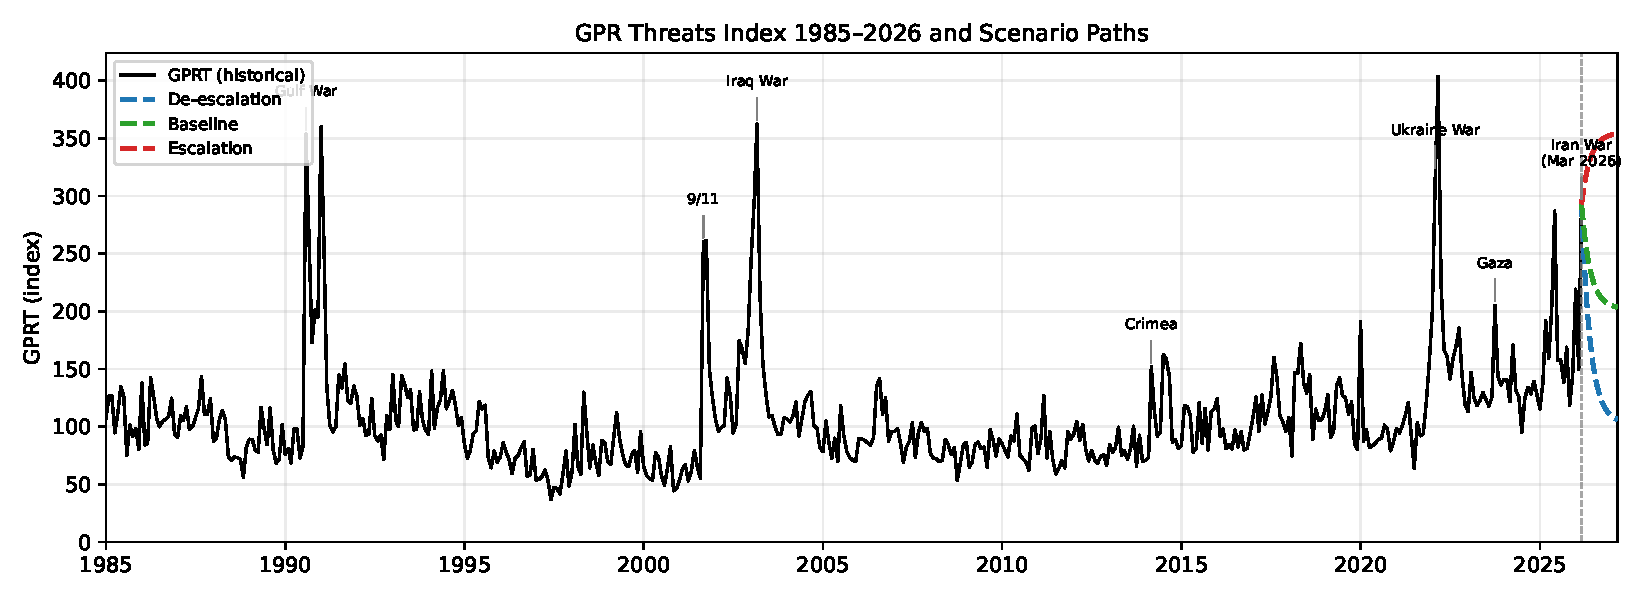
\includegraphics[width=\linewidth,height=0.60\textheight,keepaspectratio]{fig_gpr_calibration}

  \smallskip

  AR(1) mean-reversion at $\rho = 0.710$ distributes the GPR impulse
  continuously over the 12-month horizon, avoiding an artificial
  concentration of the ARX scenario effect at $h = 1$.

\end{frame}

% ══════════════════════════════════════════════════════════════════════════════
\section{Simulation Results}
% ══════════════════════════════════════════════════════════════════════════════

\iffalse
% ── Slide 8.0 (hidden) ───────────────────────────────────────────────────────
\subsection{Model Validation: Feb 2026 Forecast vs.\ March 2026 Realized}

\begin{frame}[shrink=10]{Model Validation: Feb 2026 Forecast vs.\ March 2026 Realized}

  v4 Channel~A baseline ($h=1$ from Feb 2026 P$_0$) vs.\ CMO realized March 2026
  prices --- out-of-sample directional test:

  {\footnotesize
  \begin{tabular}{lrrrr}
    \toprule
    Commodity   & v4 Base $h{=}1$ & v4 Esc $h{=}1$ & Realized (Mar 2026) & Dir.\ \\
                & (\%$\Delta$)    & (\%$\Delta$)   & (\%$\Delta$ vs.\ Feb) &      \\
    \midrule
    Crude Oil   & $+1.3$  & $+3.4$  & $\mathbf{+40.5}$ & \checkmark \\
    Brent       & $+1.3$  & $+3.4$  & $\mathbf{+45.8}$ & \checkmark \\
    NatGas US   & $-8.3$  & $-8.1$  & $\mathbf{-15.6}$ & \checkmark \\
    NatGas EU   & $+3.8$  & $+5.0$  & $\mathbf{+59.4}$ & \checkmark \\
    LNG Japan   & $-0.2$  & $-0.6$  & $\mathbf{+31.1}$ & $\times$   \\
    Coal AU     & $-2.0$  & $-1.3$  & $\mathbf{+17.1}$ & $\times$   \\
    Urea        & $-2.5$  & $-2.9$  & $\mathbf{+53.7}$ & $\times$   \\
    DAP         & $+3.0$  & $+3.5$  & $\mathbf{+5.1}$  & \checkmark \\
    TSP         & $+3.0$  & $+3.5$  & $\mathbf{+4.1}$  & \checkmark \\
    Aluminum    & $+0.8$  & $+1.8$  & $\mathbf{+10.0}$ & \checkmark \\
    \bottomrule
  \end{tabular}
  }

  \begin{alertblock}{Shock already materialized --- use realized P$_0$}
    v4 correctly predicted direction for 7/10 commodities but \emph{severely}
    under-predicted magnitude: realized energy prices ($+40$--$60\%$) dwarfed
    even the escalation $h=1$ path ($+3$--$5\%$).  The GPR shock was no longer
    a scenario --- it had occurred.  Using March 2026 as P$_0$ in v5 anchors
    projections to the post-shock market state rather than forecasting from
    pre-shock levels.
  \end{alertblock}

\end{frame}
\fi

% ── Slide 8.1 ─────────────────────────────────────────────────────────────────
\subsection{12-Month Price Forecasts: Cross-Scenario Summary}

\begin{frame}[shrink=10]{12-Month Price Forecasts: Cross-Scenario Summary}

  \medskip

  \begin{tabular}{llrrrr}
    \toprule
    Group       & Commodity   & Current      & De-escal.    & Baseline     & Escalation  \\
                &             & Mar 2026     & (\%$\Delta$) & (\%$\Delta$) & (\%$\Delta$) \\
    \midrule
    Energy      & Crude Oil   &   95.58 & $+0.0$   & $+13.0$  & $+32.9$  \\
    Energy      & Brent       &  103.69 & $+0.2$   & $+14.9$  & $+38.2$  \\
    Energy      & NatGas US   &    3.05 & $+21.3$  & $+30.6$  & $+44.0$  \\
    Energy      & NatGas EU   &   17.91 & $+17.8$  & $+35.5$  & $+66.3$  \\
    Energy      & LNG Japan   &   14.85 & $+40.6$  & $+49.6$  & $+64.3$  \\
    Energy      & Coal AU     &  138.60 & $+15.2$  & $+35.3$  & $+70.7$  \\
    Fertilizers & Urea        &  725.63 & $+30.1$  & $+50.3$  & $+87.2$  \\
    Fertilizers & DAP         &  658.25 & $+54.7$  & $+115.8$ & $+255.7$ \\
    Fertilizers & TSP         &  558.13 & $+59.4$  & $+131.8$ & $+304.6$ \\
    Fertilizers & Phosphate   &  152.50 & $+42.0$  & $+63.0$  & $+99.0$  \\
    Agriculture & Wheat       &  275.91 & $+6.2$   & $+12.2$  & $+22.4$  \\
    Agriculture & Maize       &  212.69 & $+3.4$   & $+10.3$  & $+21.1$  \\
    Metals      & Copper      & 12{,}529 & $+0.7$ & $+3.1$  & $+7.0$  \\
    Metals      & Aluminum    &  3{,}373 & $+10.8$ & $+31.3$ & $+68.9$ \\
    \bottomrule
  \end{tabular}


\end{frame}

% ── Slide 8.2 ─────────────────────────────────────────────────────────────────
\subsection{Energy: Scenario Fan Charts}

\begin{frame}{Energy: Scenario Fan Charts}

  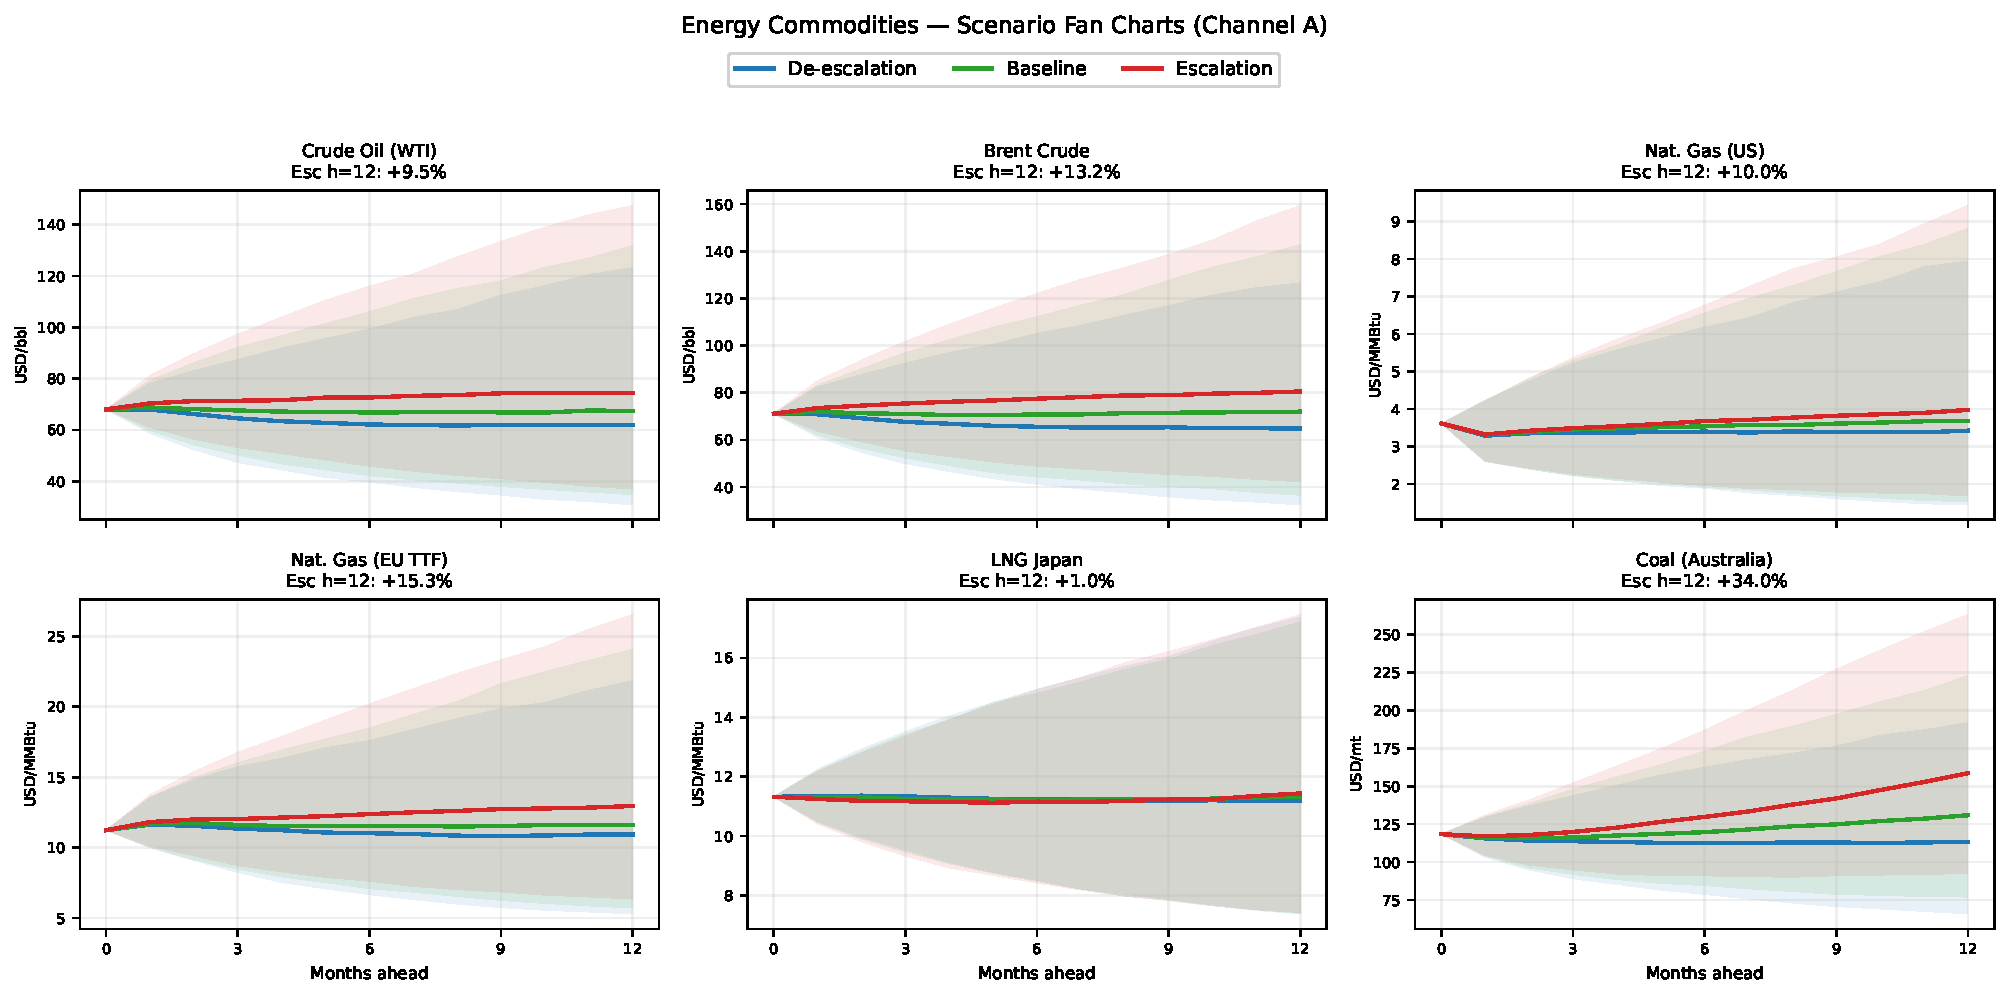
\includegraphics[width=\linewidth,height=0.80\textheight,keepaspectratio]{fig_energy_fancharts}

\end{frame}

% ── Slide 8.3 ─────────────────────────────────────────────────────────────────
\subsection{Fertilizers \& Agriculture: Scenario Fan Charts}

\begin{frame}{Fertilizers \& Agriculture: Scenario Fan Charts}

  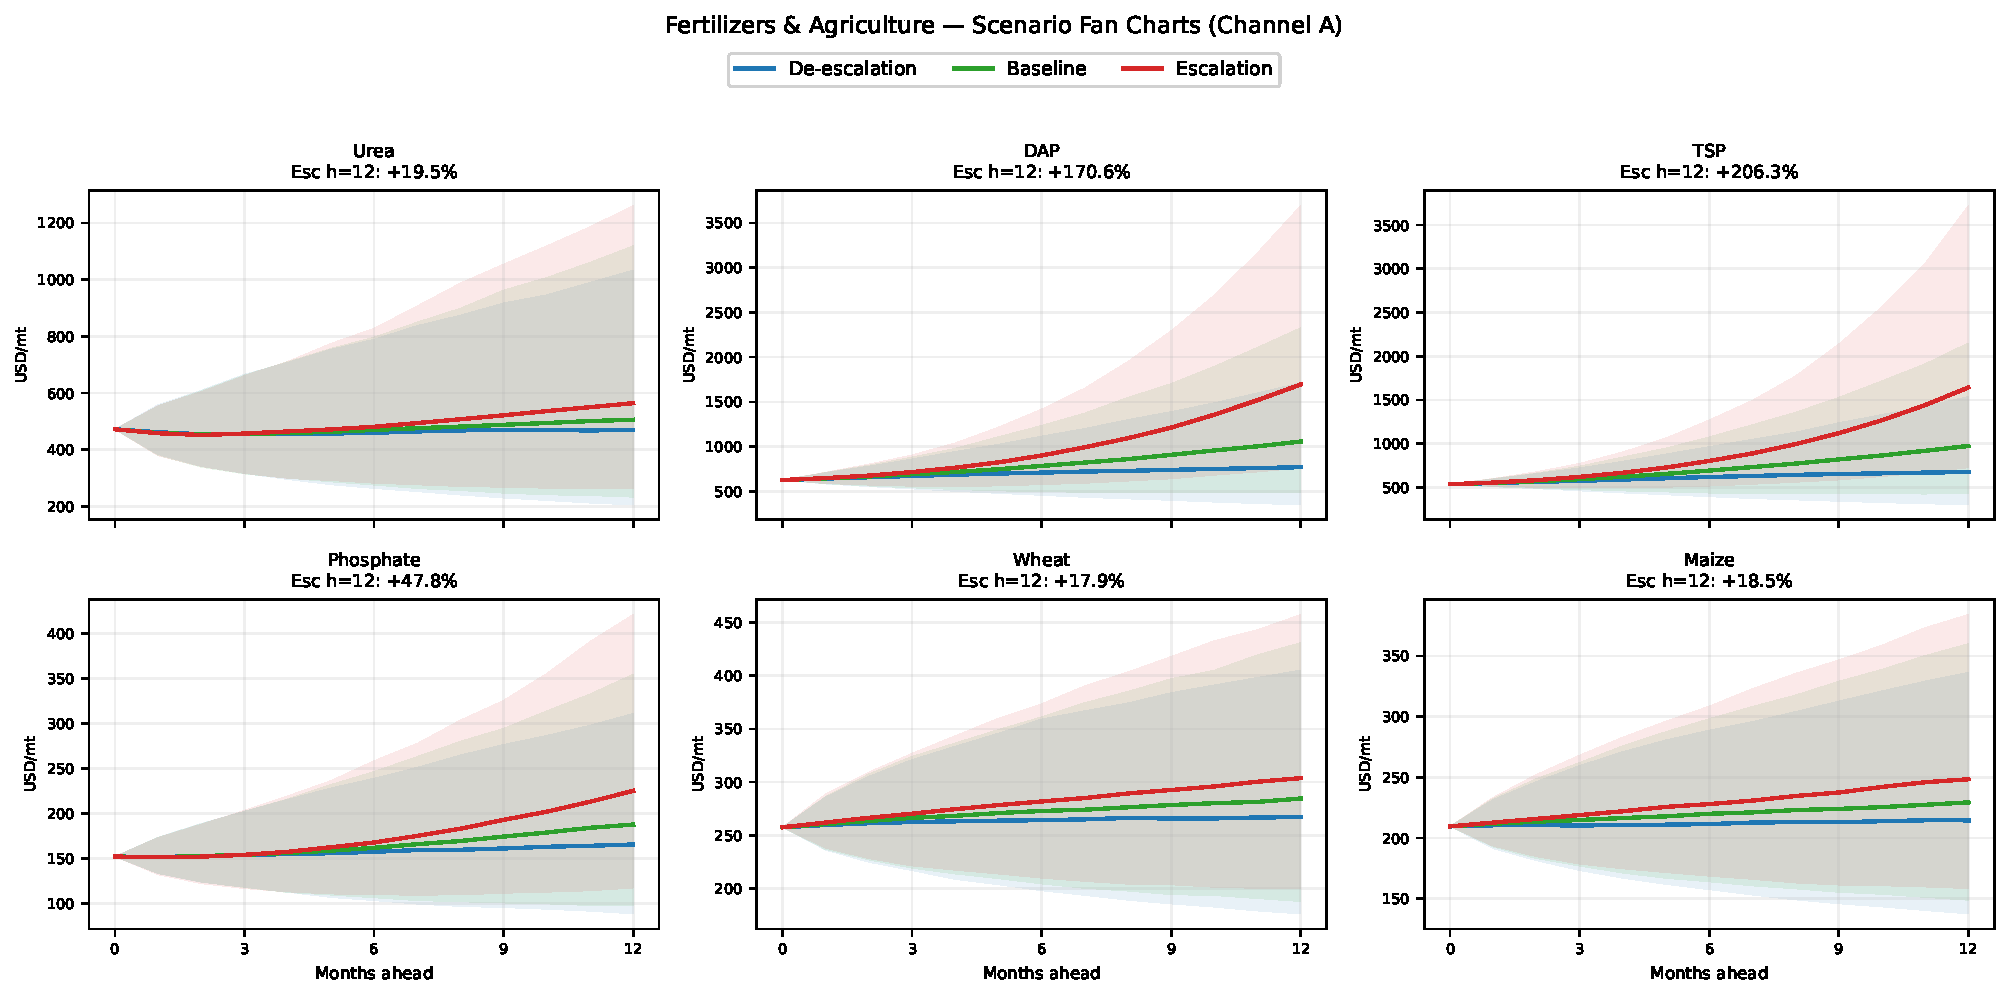
\includegraphics[width=\linewidth,height=0.80\textheight,keepaspectratio]{fig_fert_ag_fancharts}

\end{frame}

% ── Slide 8.4 ─────────────────────────────────────────────────────────────────
\subsection{Metals: Scenario Fan Charts}

\begin{frame}{Metals: Scenario Fan Charts}

  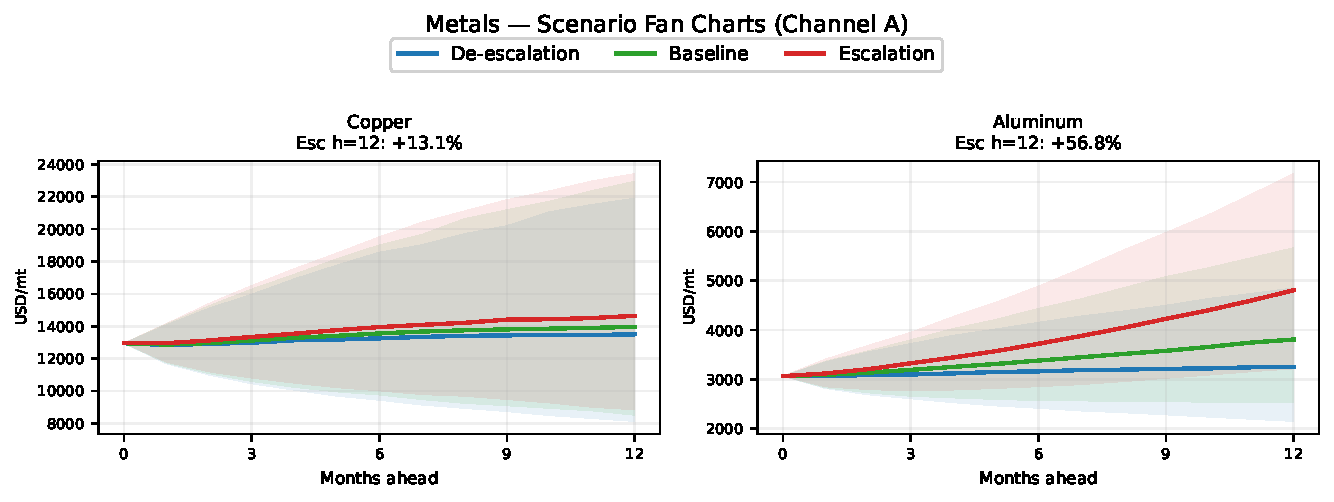
\includegraphics[width=\linewidth,height=0.80\textheight,keepaspectratio]{fig_metals_fancharts}

\end{frame}

% ── Slide 8.5 ─────────────────────────────────────────────────────────────────
\subsection{Fan Chart Commentary}

\begin{frame}[shrink=10]{Scenario Fan Charts: Key Takeaways}

  \textbf{Energy:}
  \begin{itemize}
    \item Crude oil and Brent separate clearly across scenarios
          --- direct GPR sensitivity ($\hat{\kappa}^T$ significant at 1\%)
    \item LNG Japan: scenario paths converge --- no significant GPR coefficient;
          price driven by long-term contracts
    \item Coal AU: $+70.7\%$ under escalation via AR persistence and energy
          substitution demand
  \end{itemize}

  \medskip

  \textbf{Fertilizers \& Agriculture:}
  \begin{itemize}
    \item DAP and TSP diverge sharply ($+256\%$, $+305\%$) via mutual cross-beta
          amplification --- not direct GPR sensitivity ($\hat{\kappa}^T \approx 0$)
    \item Wheat and Maize show real but moderate scenario spread
  \end{itemize}

  \medskip

  \textbf{Metals:}
  \begin{itemize}
    \item Aluminum: strongest direct GPR sensitivity ($p = 0.003$); $+68.9\%$
          under escalation via energy-intensive electrolytic smelting
    \item Copper: marginal GPR sensitivity; moderate escalation response
  \end{itemize}

\end{frame}

% ── Slide 8.6 ─────────────────────────────────────────────────────────────────
\subsection{Fertilizer Indirect Transmission: Network Decomposition}

\begin{frame}[shrink=10]{Fertilizer Indirect Transmission: Network Decomposition}

  Escalation vs Baseline, $h = 12$ --- pp gap (Esc $-$ Base) decomposed into
  GPR-direct vs network-propagated components (\texttt{v5\_koyck\_mar2026};
  network/direct split uses v4 structural shares):

  {\footnotesize
  \begin{tabular}{lrrrr}
    \toprule
    Commodity      & Full (pp) & Direct GPR (pp) & Network (pp) & Net share \\
    \midrule
    CrudeOil ***   & $+19.9$ & $+16.9$ & $+3.0$  & $15\%$ \\
    Brent ***      & $+23.3$ & $+20.3$ & $+3.0$  & $13\%$ \\
    Aluminum **    & $+37.6$ & $+26.0$ & $+11.7$ & $31\%$ \\
    Coal AU        & $+35.4$ & $+34.0$ & $+1.4$  & $ 4\%$ \\
    NatGas EU      & $+30.8$ & $+24.3$ & $+6.5$  & $21\%$ \\
    DAP            & $+139.9$& $+36.4$ & $+103.5$& $74\%$ \\
    TSP            & $+172.8$& $+50.1$ & $+122.7$& $71\%$ \\
    Phosphate      & $+36.0$ & $+2.2$  & $+33.8$ & $94\%$ \\
    Urea           & $+36.9$ & $+14.4$ & $+22.5$ & $61\%$ \\
    Wheat          & $+10.2$ & $+10.2$ & $\approx0$ & $0\%$ \\
    \bottomrule
  \end{tabular}
  }

  \begin{alertblock}{Second-order energy shock}
    For DAP and TSP the network share is \textbf{74\%} and \textbf{71\%}; Phosphate
    reaches \textbf{94\%}.  Energy commodities show only 13--21\% network share
    (mostly direct GPR).  The fertilizer price spike is a delayed, amplified
    consequence of the energy shock --- statistically grounded, not a model artefact.
  \end{alertblock}

\end{frame}

% ══════════════════════════════════════════════════════════════════════════════
\section{Country Impact}
% ══════════════════════════════════════════════════════════════════════════════

% ── Slide 9.1 ─────────────────────────────────────────────────────────────────
\subsection{Comtrade Trade-Balance Methodology}

\begin{frame}[shrink=10]{Country Exposure: Methodology}

  \begin{itemize}
    \item \textbf{Source:} UN Comtrade bilateral trade flows, 2021--2023 three-year average
    \item \textbf{Net exposure:} (imports $-$ exports) / total bilateral trade
          per commodity--country pair
    \item Positive net exposure = net importer: price rise is a cost to the
          trade balance
    \item Negative net exposure = net exporter: price rise is a gain
    \item Natural gas: consolidated into a single composite series (average of
          NatGas US and NatGas EU price paths) to avoid double-counting from
          HS code 2711 shared by both benchmarks
    \item \textbf{Exposure index:}
          $\sum_i w_i \cdot \hat{P}_i^{\,\text{Escalation}}$,
          where $w_i$ is the net trade share
  \end{itemize}

  \begin{alertblock}{Scope}
    Trade-balance exposure captures the first-order macro impact under the
    escalation scenario --- the commodity cost shock to each economy's import bill.
    Credit-risk and financial contagion channels are not modelled.
  \end{alertblock}

\end{frame}

% ── Slide 9.2 ─────────────────────────────────────────────────────────────────
\subsection{Country Exposure Under Escalation}

\begin{frame}[shrink=25]{Country Exposure Under Escalation}

  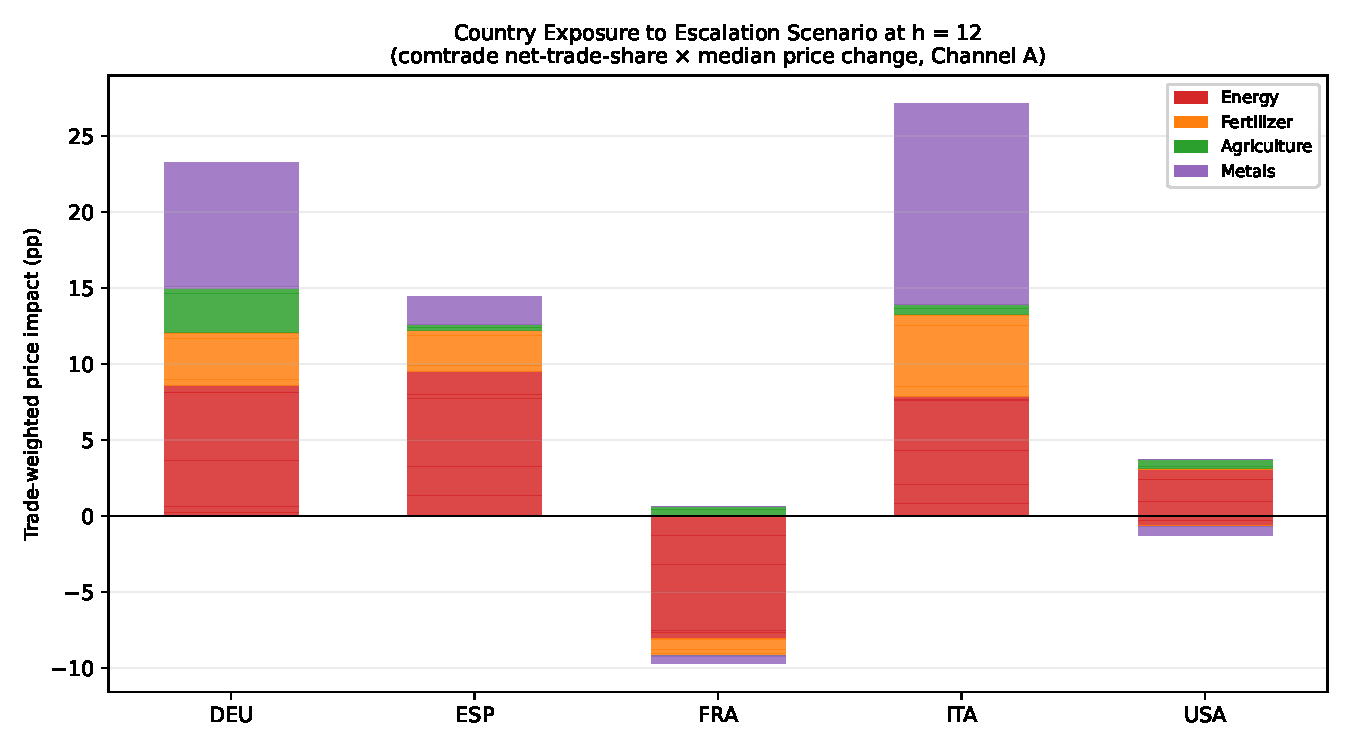
\includegraphics[width=\linewidth,height=0.55\textheight,keepaspectratio]{fig_country_exposure}

  \smallskip

  \begin{tabular}{lll}
    \toprule
    Country & Role & Dominant exposure \\
    \midrule
    DEU & Net energy importer & Large: NatGas EU, Coal, Fertilizers \\
    ITA & Net energy importer & Similar to DEU; fertilizer-intensive \\
    ESP & Net energy importer & Oil and gas dominant \\
    FRA & Mixed               & Oil importer, partially nuclear-insulated \\
    USA & Net energy exporter & Negative energy bars offset import costs \\
    \bottomrule
  \end{tabular}

  \smallskip

  Under escalation at $h = 12$, net-importing European economies face
  exposure-weighted commodity basket increases of $+31.0\%$ (DEU), $+37.6\%$ (ITA),
  and $+36.4\%$ (ESP).  France, partially insulated by nuclear energy, registers a
  $-23.8\%$ net cost change: France is a large net agricultural exporter
  (wheat, maize) in the Comtrade basket, whose grain-export gains under rising
  prices more than offset its crude oil and gas import costs.  The USA, a net energy
  exporter, faces only $+6.2\%$.  (\texttt{v5\_koyck\_mar2026}, Comtrade weights.)

\end{frame}

% ══════════════════════════════════════════════════════════════════════════════
\section{Conclusions}
% ══════════════════════════════════════════════════════════════════════════════

% ── Slide 10.1 ────────────────────────────────────────────────────────────────
\subsection{Key Findings and Limitations}

\begin{frame}[shrink=10]{Key Findings and Limitations}

  \begin{itemize}
    \item Crude oil responds asymmetrically: GPRT threat raises prices
          (risk premium); GPRA act lowers them (demand destruction) ---
          \emph{buy the rumour, sell the news}
    \item \textbf{Fertilizers} are the most vulnerable commodity under escalation
          (DAP $+256\%$, TSP $+305\%$), driven predominantly by indirect network
          propagation (74\% and 71\% network shares), not direct GPR sensitivity
    \item Geopolitical crises \textbf{decouple} cross-sector correlation
          ($\hat{\beta}_T < 0$): the independence assumption is approximately
          correct for cross-sector pairs under stress
    \item Under escalation, European net importers face 30--40\% commodity cost
          increases over 12 months (DEU $+31\%$, ITA $+38\%$, ESP $+36\%$)
  \end{itemize}

  \textbf{Limitations:}
  \begin{itemize}
    \item Fertilizer channel relies on cross-beta network stability
    \item DCC ARCH $\approx 0$: correlation dynamics are regime-level, not
          shock-level
    \item GPR scenario paths are deterministic (AR(1) mean); GPR uncertainty
          is not propagated
  \end{itemize}

  \begin{alertblock}{}
    The three-layer model is not a black-box forecast. Each layer produces an
    independent, interpretable finding about commodity price dynamics under
    geopolitical stress.
  \end{alertblock}

\end{frame}

% ── References ────────────────────────────────────────────────────────────────
\begin{frame}[allowframebreaks]{References}
  \printbibliography
\end{frame}

\end{document}